\documentclass{article}

%% Denote paragraphs with vertical space rather than indenting (not critical)
\usepackage{parskip}

%% Support for URL in introductory text (not needed for main example)
\usepackage{url}

%% *** Enable TikZ ***
\usepackage{tikz}


\begin{document}

%% Introductory Text
Example 3.4 from the book\\
\emph{Unlocking LaTeX Graphics: A Concise Guide to Ti$k$Z/PGF and PGFPLOTS}.\\
For more information, visit \url{https://latex-graphics.com}.
\par\bigskip

%% *** START OF EXAMPLE CODE ***
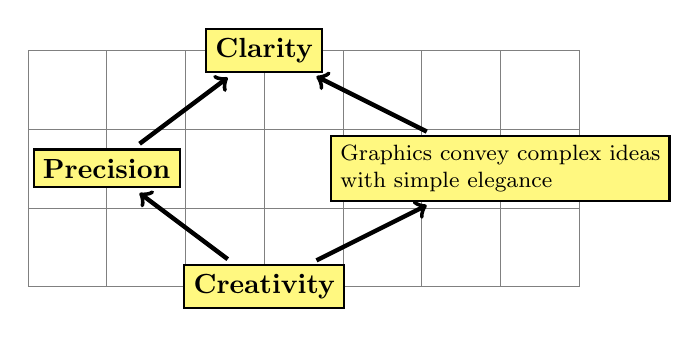
\begin{tikzpicture}[
    every node/.style={draw,thick,fill=yellow!50,font=\bfseries,align=left},
    arw/.style={ultra thick,shorten >=1mm,shorten <=1mm,->}]
  \draw[help lines] grid(7,3);
  \node (Precision) at (1,1.5) {Precision};
  \node at (3,0) (Creativity) {Creativity};
  \node at (3,3) (Clarity) {Clarity};
  \node[font=\footnotesize] at (6,1.5) (Graphics) {Graphics convey complex ideas\\ with simple elegance};
  \draw[arw] (Precision) -- (Clarity);
  \draw[arw] (Graphics) -- (Clarity);
  \draw[arw] (Creativity) -- (Graphics);
  \draw[arw] (Creativity) -- (Precision);
\end{tikzpicture}
%% *** END OF EXAMPLE CODE ***

\end{document}
